%%%%%%%%%%%%%%%%%%%%%%%%%%%%%%%%%%%%%%%%%%%%%%%%%%%%%%%%%%%%%%%%%%%%
%PLANTILLA DE INFORMES V 1.1
%
% REQUISITO: IMPORTE EL LOGO DE LA USM CON EL NOMBRE "logousm.png"
% IMPORTE IMAGENES DE MODULOS, EXTRAER DEL WORD
%
% Material de referencia de proposito general:
% https://users.dcc.uchile.cl/~jbarrios/latex/
% http://mate.dm.uba.ar/~pdenapo/tutorial-latex/node2.html
% http://tiburondealambre.blogspot.cl/2012/01/referencias-imagenes-y-tablas-en-latex.html
% BIBLIOGRAFIA: http://logistica.fime.uanl.mx/miguel/docs/BibTeX.pdf
%
% Tratar ecuaciones en latex(muy util):
% https://ondiz.github.io/cursoLatex/Contenido/05.Ecuaciones.html
%
% detector de cosas dibujadas latex: http://detexify.kirelabs.org/classify.html
%
%%%%%%%%%%%%%%%%%%%%%%%%%%%%%%%%%%%%%%%%%%%%%%%%%%%%%%%%%%%%%%%%%%%%%%%

%----------------------PAQUETES---------------------------%
% No es necesario tocar nada de esto

\documentclass[12pt,a4paper]{article} % tipo de documento, formato

\usepackage[utf8]{inputenc}    % con tildes
\usepackage[spanish]{babel}    % arreglar problemas

\usepackage[framed,numbered,final]{mcode} %%MATLAB

\usepackage{hyperref}

\usepackage{graphicx} % paquete de tratado de imagenes/figuras
\usepackage{tipa} % para <
\usepackage{amssymb} % para >=

% paquete extra para ocupar [H] (obliga a que la imagen con graphicx
% se quede donde se realizó el llamado)
\usepackage{float}

% CARGAMOS 3 PAQUETES
% (AMS Math), que mejora el comportamiento y el aspecto de las ecuaciones. 
% Nos permite, por ejemplo, añadir un asterisco en el entorno equation para crear
% ecuaciones sin numerar.
%(AMS Theorem), que define los entornos teorema y demostración.
%(AMS Symbol), que carga a su vez amsfonts e incluye una colección 
%de símbolos matemáticos.
\usepackage{amsmath, amsthm, amssymb} 

\usepackage{enumerate} %permite enumerar de varias formas

\usepackage{multirow, array} % para las tablas

% construccion de un nuevo comando
\usepackage{lipsum}% http://ctan.org/pkg/lipsum
\usepackage{xcolor}% http://ctan.org/pkg/xcolor
\usepackage{xparse}% http://ctan.org/pkg/xparse
\NewDocumentCommand{\myrule}{O{1pt} O{2pt} O{black}}{%
  \par\nobreak % don't break a page here
  \kern\the\prevdepth % don't take into account the depth of the preceding line
  \kern#2 % space before the rule
  {\color{#3}\hrule height #1 width\hsize} % the rule
  \kern#2 % space after the rule
  \nointerlineskip % no additional space after the rule
}

%acomoda margenes y tipografia para que quede mas bonito
\usepackage{geometry}
\geometry{
	paper=a4paper, % Change to letterpaper for US letter
	inner=3cm, % Inner margin
	outer=3cm, % Outer margin
	bindingoffset=.5cm, % Binding offset
	top=2cm, % Top margin
	bottom=2cm, % Bottom margin
	%showframe, % Uncomment to show how the type block is set on the page
}


%---------PORTADA, TABLA DE CONTENIOS Y FIGURAS--------------%
%Esto será la portada. Solo hay que cambiar los textos
\begin{document}

\begin{titlepage}
\begin{center}
\textbf{\LARGE Universidad Técnica Federico Santa}\\[0.25cm]
\textbf{\LARGE María}\\[0.5cm]
\textbf{\large DEPARTAMENTO DE INGENIERÍA ELECTRONICA}\\[0.2cm]
\vspace{20pt}
\includegraphics{logousm.png}\\[1cm]

\par
\vspace{15pt}
\textbf{\Large ELO 314 - Laboratorio de procesamiento Digital de Señales}\\
\vspace{15pt}
\myrule[1pt][7pt]
\textbf{\LARGE Proyectos en LCDK y Recomendaciones Practicas }\\[0.25cm]
\vspace{15pt}
\textbf{\large  }\\
\myrule[1pt][7pt]
\vspace{55pt}
\textbf{\large Estudiante \hspace{75pt} ROL}\\
    \hspace{0pt}Rodrigo Graves\hspace{80pt} 201621009-1 \\
     Ricardo Mardones      \hspace{60pt} 201621036-9 \\
   


\vspace{30pt}
\textbf{\large Paralelo: \hspace{30pt} 1}\\

\vspace{35pt}
\textbf {\large Profesor}\\[0.2cm]
\Large { Gonzalo Carrasco}\\[0.1cm]
\textbf {\large Ayudante}\\[0.2cm]
\Large {Jaime Guzmán}\\[0.1cm]
\end{center}

\par
\vfill
\begin{center}
\textbf{Fecha : \today}\\
\end{center}

\end{titlepage}


%-------------Lista de figuras y tablas----------%
\tableofcontents % Hace el índice de contenidos. Latex organiza todo solito
\listoffigures %lista de figuras
\listoftables


\newpage


\section{Configuración de proyecto ejecutable: CCS}

\begin{enumerate}
    \item  Se importa el proyecto de la carpeta \textit{lab0/build} al IDE ccs entregada junto con el repositorio del curso. Una vez importado, al intentar efectuar la construcción haciendo click en \textit{build proyect} lo que se obtiene es una serie de errores y mensajes de \textit{warnings}
    
    
    Entre ellos se indica que la ruta hacia los archivos del proyecto importado, en la sección referente a la compilación, no es accesible pues indica directorios que no pertenecen al dispositivo en el que se está trabajando. Las que se indican en el proyecto inicialmente se muestran en la figura \ref{path_profe}
    
    
    \begin{figure}[H]
        \centering
        \includegraphics[width = 0.9 \linewidth]{figures/pathProfe.png}
        \caption{Configuración inicial del compilador con las rutas ajenas.}
        \label{path_profe}
    \end{figure}
    
    
    Modificando las rutas hacia la ubicación local de los archivos y añadiendo además la ruta hacia el directorio \textit{DSP\_AIC3016} , ya que también existían errores indicando que requiere archivos ubicados en ese directorio  (ver figura \ref{error}), la  sección \textit{Build C000 Linker Include Options} de configura como se muestra en la figura \ref{path_local}
    
    
    
    \begin{figure}[H]
        \centering
        \includegraphics[scale = 0.8]{figures/error_aic3106.png}
        \caption{Error referente a la falta del directorio \textit{DSP\_AIC3016}}
        \label{error}
    \end{figure}
    \begin{figure}[H]
        \centering
        \includegraphics[scale = 0.5]{figures/path_local.png}
        \caption{Configuración del compilador con las ruta locales de trabajo.}
        \label{path_local}
    \end{figure}
    
    
    Por otro lado, se debe añadir la una dependencia extra en la sección \textit{linker}, dado que inicialmente solo se encuentra una por defecto en el proyecto, esto se muestra en la figura \ref{liker}
    
    \begin{figure}[H]
        \centering
\includegraphics[scale = 0.3]{figures/linker_profe.png}
        \caption{Configuración inicial del \textit{linker} del proyecto.}
        \label{liker}
    \end{figure}
    
    
    Luego de añadir la dependencia necesaria la configuración queda de la siguiente forma
    
    \begin{figure}[H]
        \centering
        \includegraphics[scale = 0.5]{figures/linker_local.png}
        \caption{Configuración del \textit{linker} del proyecto con dependencias ya añadidas.}
        \label{fig:my_label}
    \end{figure}
    
    
    
    Para solucionar el último error que impide la construcción correcta del proyecto se añade manualmente el archivo \textit{L138\_LCDK\_aic3106\_init.c} utilizando la ruta local de dicho archivo.
    
    
    \begin{figure}[H]
        \centering
        \includegraphics[scale = 0.5]{figures/aic3106.png}
        \caption{Se añade archivo \textit{L138\_LCDK\_aic3106\_init.c} requerido para construcción correcta del proyecto.}
        \label{fig:my_label}
    \end{figure}
    
    
    La figura \ref{correct_build} muestra como se ha logrado la correcta construcción del proyecto con las configuraciones hechas
    
    \begin{figure}[H]
        \centering
        \includegraphics[scale = 0.7]{figures/correct_build.png}
        \caption{Construcción exitosa del proyecto }
        \label{correct_build}
    \end{figure}
    
    
    
\end{enumerate}
\clearpage


\newpage
\section{Inclusión de librería a un proyecto: MATHLIB}


El proyecto sobre el cual se está trabajando utiliza en una de sus lineas la función \textit{cosf()} incluida desde la librería \textit{math.h}, sin embargo dado que es un proyecto pensado para ser implementado en una tarjeta LCDK que cuenta con un procesador de núcleo \textit{C674x}, es recomendable reemplazar dicha función por alguna provista por la librería \textit{MATHLIB}, que es recomendada por los fabricantes Texas Instrument (TI), en este caso se hará uso de la función \textit{cossp()}  (coseno \textit{single-precision}, para \textit{float} según MATHLIB).


Para esto se deben realizar algunos cambios en las configuraciones de compilación y enlace del proyecto. Primero se deben añadir las rutas que dirijan a los paquetes de la librería MATHLIB, como se muestran la figura \ref{path_mathlib}




\begin{figure}[H]
    \centering
    \includegraphics[scale = 0.6]{figures/mathlib_compiler.png}
    \caption{Configuración adicional al compilador para usar la librería MATHLIB}
    \label{path_mathlib}
\end{figure}


 Además se debe agregar la dependencia \textit{mathlib.lib}, indicando claramente el directorio en que se encuentra, esto se indica en la figura \ref{linker_mathlib}

\begin{figure}[H]
    \centering
    \includegraphics[scale = 0.6]{figures/mathlib_linker.png}
    \caption{Configuración adicional al \textit{linker} para usar la librería MATHLIB}
    \label{linker_mathlib}
\end{figure}

Además en la sección de inclusión de librerías del código en el archivo \textit{L1P2.c} se debe agregar la linea \texttt{\#include  ``mathlib.h''} y se debe modificar la línea 142 del código


\begin{lstlisting}[frame = single]
#include "mathlib.h"

...

...

%linea original
cosSignal = (int16_t)( 2 * ampCosine * cosf(thetaCosineSignal) );

%linea modificada
cosSignal = (int16_t)( 2 * ampCosine * cossp(thetaCosineSignal) );
\end{lstlisting}


Revisando la documentación asociada a la librería MATHLIB posee diversas funciones que permiten trabajar de forma sencilla con elementos matemáticos, entre ellas funciones trigonométricas, logaritmos, exponenciales, y potencias. Todas estas implementadas tanto para trabajar con datos de precisión simple y doble, permitiendo una versatilidad para diversas arquitecturas al trabajar con distinto número de bits.

Esto resulta beneficioso ya que al estar estas funciones ya implementadas en una librería se reduce considerablemente el tiempo de procesamiento al momento de ejecutar operaciones matemáticas al trabajar con enfoques en tiempo real.




\clearpage

\section{Estudio de la API de una librería: DSPLIB}

\begin{enumerate}
    \item  La librería \textit{DSPLIB} provee una serie de funciones diseñadas y optimizadas para facilitar el procesamiento digital de señales en tarjetas físicas, simplificando la implementación en lenguaje C, que suele ser el utilizado en este tipo de dispositivos. El que dichas funciones estén optimizadas con un objetivo claro permite reducir el tiempo de ejecución necesario para este tipo de procesamientos, que suele ser un punto de consideración al desarrollar proyectos que trabajen en tiempo real. Algunas de estas funciones se listan a continuación



\begin{itemize}
    
    \item \textbf{DSPF\_sp\_biquad:} Realiza  filtrado de una señal usando un filtro biquad.
    \item \textbf{DSPF\_sp\_convol:} Efectúa la convolución entre dos arreglos de entrada.
    \item \textbf{DSPF\_sp\_fir\_gen:} Realiza  filtrado FIR a una matriz de entrada  a partir de vectores con los coeficientes del filtro.
    \item \textbf{DSPF\_sp\_iir:}  Realiza  filtrado IIR a una matriz de entrada  a partir de vectores con los coeficientes del filtro.
    \item \textbf{DSPF\_sp\_mat\_mul:} Multiplica dos matrices de entrada 
    
\end{itemize}


\item A continuación se detalla la forma de uso de algunas de las funciones antes mencionadas



 \textbf{DSPF\_sp\_biquad} \\
    Esta función realiza el filtrado de una señal cuyas muestras se  almacenan en un arreglo, recibe seis parámetros en su implementación. La señal resultante se almacena en el arreglo \textit{y} y la función no devuelve ningún valor (\textit{void}) pues trabaja directamente con punteros a los parámetros.
    
\\
    
\textbf{Prototipo función}    

\begin{lstlisting}
void DSPF_sp_biquad(float *restrict x, float *b, float *a,
                    float *delay, float *restrict y, const int n)
\end{lstlisting}

\textbf{Parámetros}

\begin{itemize}
    \item float $*$x:  Puntero al arreglo de entrada  cuyo largo debe ser  \textit{n}, donde n corresponde al último de los parámetros requerido por la función y que se describe a continuación.
    \item float $*$b: Puntero al arreglo de coeficientes $B_k$ del filtro biquad cuyo largo debe ser  3. En este arreglo los coeficientes deben aparecer en el orden  {$b_0$, $b_1$, $b_2$}
    \item float $*$a:  Puntero al arreglo de coeficientes $A_k$ del filtro biquad cuyo largo debe ser  3. En este arreglo los coeficientes deben aparecer en el orden  {$a_0$, $a_1$, $a_2$}
    \item float $*$delay: Puntero arreglo de coeficientes de retraso asociado al filtro. Debe tener largo 2.
    \item float $*$y: Puntero al arreglo de valores de salida cuyo largo debe ser \textit{n},  donde n corresponde al último de los parámetros requerido por la función y que se describe a continuación.
    \item const int n: Largo de los arreglos de entrada y de salida. Debe ser un número par.
\end{itemize}


    
\textbf{DSPF\_sp\_mat\_mul}

\\ \\

La función realiza la multiplicación de dos matrices de entrada, cuyas dimensiones deben ser consistentes para poder ser multiplicadas. El resultado se almacena en la matriz de salida \textit{y} y la función no retorna nada (\textit{void}) pues trabaja directamente con los punteros a los parámetros.

\textbf{Prototipo función}    

\begin{lstlisting}
void DSPF_sp_mat_mul(float *x1, const int r1, const int c1, 
                float *x2, const int c2, float *restrict y)

\end{lstlisting}

\textbf{Parámetros}

\begin{itemize}
    \item float $*$x:  Puntero a la primera matriz de entrada, de $r1 \cdot c1$ elementos.
    \item const int r1: Número de filas de la primera matriz de entrada.
    \item const int c1: Número de columnas de la primera matriz de entrada.

    \item float $*$x2: Puntero a la segunda  matriz de entrada, de $c1 \cdot c2$ elementos.
    \item const int c2:Número de columnas de la segunda matriz de entrada.
    
     \item *restrict y: Puntero a la matriz resultante a partir de la multiplicación, el tamaño de este resultado es de $r1$ filas y $c2$ columnas.
\end{itemize}


\end{enumerate}
\clearpage

\section{Mediciones de validación de proyecto de ejemplo: Phaser}

\subsection{Prueba diseñada:}

Los pasos propuestos para validar el correcto funcionamiento del efecto phaser en la LCDK son los que se presentan a continuación:

\begin{enumerate}
    \item Con la placa LCDK programada en modo bypass, usar de señal de entrada al codec de audio una señal de ruido blanco (y por lo tanto de espectro distribuido) de 1 Vpp obtenido a partir de un generador de señales.
    
    Este es importante por 2 razones:
    \begin{itemize}
        \item Verificar el funcionamiento del modo bypass.
        \item Contar con señal de referencia para futuras comparaciones.%La señal de ruido blanco es de espectro distribuido, por lo que en el espectro del ruido filtrado se podrá apreciar la respuesta en frecuencia del filtro que se está usando en un momento en particular.
    \end{itemize}
    
    Se utiliza una señal de 1 Vpp para no dañar el codec.
    
    \item Importar archivo de audio en MATLAB y obtener su espectrograma con el script \texttt{Spectrogram\_test}, previamente implementado.
    
    El espectrograma permitirá verificar que la señal sea de espectro distribuido en el tiempo
    
    \item Repetir paso 1 con phaser activado.
    
    El espectro de está señal se verá afectado por el filtro dinámico.
    
    \item Importar archivo de audio grabado en paso anterior en MATLAB y obtener su espectrograma con el script del paso 2.
    
    En el espectrograma se apreciarpa el movimiento de los nulos el filtro notch en el tiempo, por lo que el funcionamiento del phaser quedará validado.
    
\end{enumerate}
\subsection{Resultados de Validación:}
Para esta parte se utilizó el código \texttt{Spectrogram\_test}.

El espectrograma de la señal de ruido blanco pasada por la LCDK en modo bypass se muestra en a figura \ref{fig:bypass}. Se aprecia el espectro plano esperado, salvo por otro lado se observa una caída en el espectro en torno a los 8 kHz. Esta caída se debe a que el códec de audio posee un filtro pasabajos a la frecuencia de Nyquist ($\tfrac{16}{2}$ kHz) con el fin de evitar los efectos de doblaje en frecuencia.  
\begin{figure}[H]
    \centering
    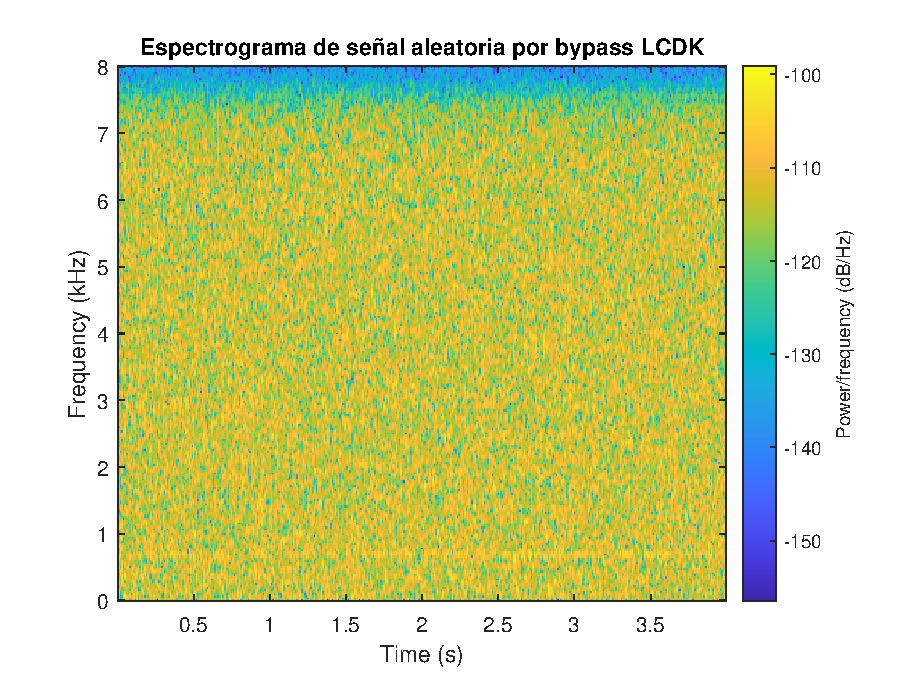
\includegraphics[width = .8\linewidth]{figures/bypass_spectrogram.eps}
    \caption{Espectrograma de señal de ruido blanco pasada por la LCDK programada en modo bypass. Ventanas 20 ms sin overlap.}
    \label{fig:bypass}
\end{figure}

El espectrograma de la señal de ruido blanco pasada por la LCDK en modo phaser se muestra en a figura \ref{fig:bypass}. Se aprecia el cambio de la frecuecias atenuadas por el filtro notch en el tiempo, por lo que se valida el correcto funcionamiento del efecto de audio.

\begin{figure}[H]
    \centering
    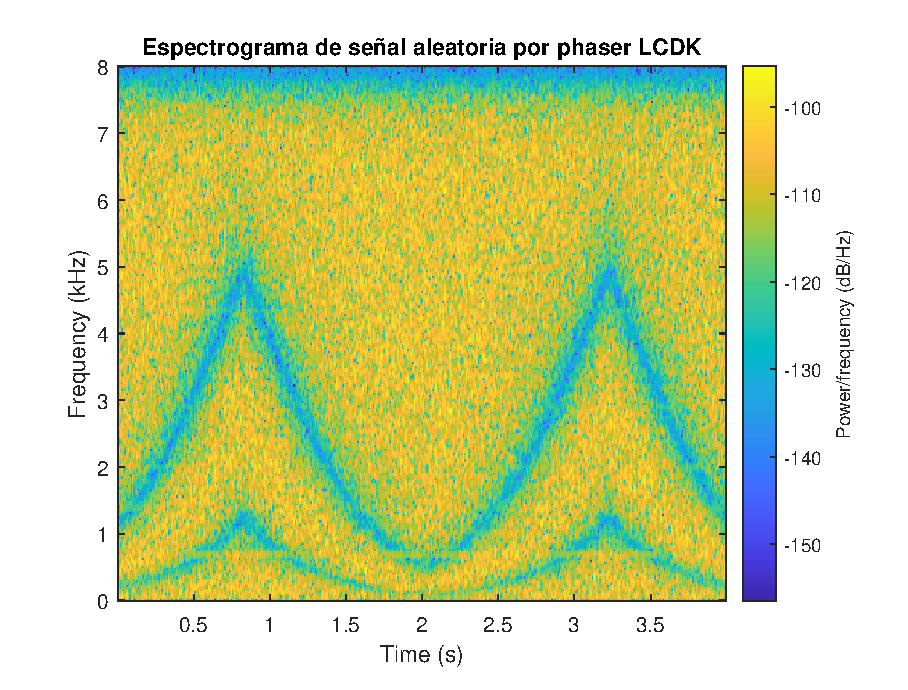
\includegraphics[width = .8\linewidth]{figures/phaser_spectrogram.eps}
    \caption{Espectrograma de señal de ruido blanco pasada por la LCDK programada en modo phaser. Ventanas 20 ms sin overlap.}
    \label{fig:phaser}
\end{figure}



\clearpage

\section{Filtro de efecto de audio dentro del \textit{codec} de audio y configuración}



\begin{enumerate}
    \item  Antes de intentar hacer uso del  \textit{codec} se debe indagar sobre las características y forma de utilizar el método de filtrado que este dispositivo incluye. Para esto se recurre al \textit{datasheet} de la tarjeta la \href{https://www.ti.com/lit/ds/symlink/tlv320aic3106.pdf?ts=1628519638980&ref_url=https}{TLV320AIC3106}  provisto por Texas Instrument \footnote{Ver en \href{https://www.ti.com/lit/ds/symlink/tlv320aic3106.pdf?ts=1628519638980&ref_url=https}{https://www.ti.com/lit/ds/symlink/tlv320aic3106.pdf?ts=1628519638980&ref_url=https} }.
    
    En la sección \textbf{10.3.3.3.1 Digital Audio Processing for Playback} se describe la estructura del filtro y como programar el bloque asociado para poder utilizarlo en un proyecto. El filtro consta de dos filtros biquad en cascada, cuyos parámetros son modificables a conveniencia y se rigen por la siguiente ecuación 
    
    
    
    $$   H(z) = \left (\frac{N_0 + 2\cdot N_1 \cdot z^{-1} + N_2 \cdot z^{-2}}{ 32768 - 2\cdot D_1 \cdot z^{-1} - D_2 \cdot z^{-2}} \right ) \cdot   \left (\frac{N_3+ 2\cdot N_4 \cdot z^{-1} + N_5 \cdot z^{-2}}{ 32768 - 2\cdot D_4 \cdot z^{-1} - D_4 \cdot z^{-2}} \right ) $$
    
    
    Donde tal como se mencionó se tiene libertad para definir los parámetros \textit{N0-5} y \textit{D0-5} asociados a ambos filtros. Además se debe tener en cuenta el signo en los parámetros dado que la expresión que se ha usado a lo largo de este curso para el diseño e implementación de filtros biquad difiere con la descrita en el \textit{datasheet}
    
    $$ H(z) = \left (\frac{b_0 + 2\cdot b_1 \cdot z^{-1} + b_2 \cdot z^{-2}}{ 1 - 2\cdot a_1 \cdot z^{-1} - a_2 \cdot z^{-2}} \right )$$
    
    
    Otra sección relevante del \textit{datasheet}  es la \textbf{10.6 Register Maps} la que describe la forma en que se guardan los parámetros definidos en los registros de memoria del dispositivos, donde se indica que los parámetros se dividen  en dos registros, cada uno de 8 bits para poder abarcar el rango $[-32768, 32768]$
    
    Finalmente resulta útil conocer como modificar la amplitud de la salida generada por el dispositivo, esto se encontró en la sección \textbf{ 10.6.1 Output Stage Volume Controls} y será relevante para el proceso que se describirá a continuación.
    
    \item Se implementa en MATLAB un script que permite encontrar los coeficientes de los filtros biquad con el fin de obtener una respuesta suficientemente cercana a la respuesta en frecuencia deseada. Cabe destacar que por la limitante impuesta por el número de bits se debe corregir la amplitud  de uno de los filtros para poder trabajar dentro del rango de valores permitido, en este caso se corrige multiplicando por un factor de 0.8 veces.

\newpage    
    \begin{lstlisting}

%Coeficientes del filtro de orden 4
F = [0 221 1764 4410 6615 8820 22050]/22050;
%correccion para entrar en [-32768, 32768]
A_corr = [2.1 2 1.3 1 1 1.2 1.5]*0.8;


%obtencion de coeficientes
[b,a] = yulewalk(4,F,A_corr);

[h,w] = freqz(b,a);


%obtencion de coeficientes para los filtros
[sos, g] = tf2sos(b,a);

b1 = sos(1,1:3)
a1 = sos(1,4:6)

b2 = sos(2,1:3)
a2 = sos(2,4:6)

\end{lstlisting}


En la figura \ref{freqz} se pueden ver las gráficas obtenidas para la respuesta en frecuencia ideal y la respuesta en frecuencia generada con el script.

\begin{figure}[H]
    \centering
    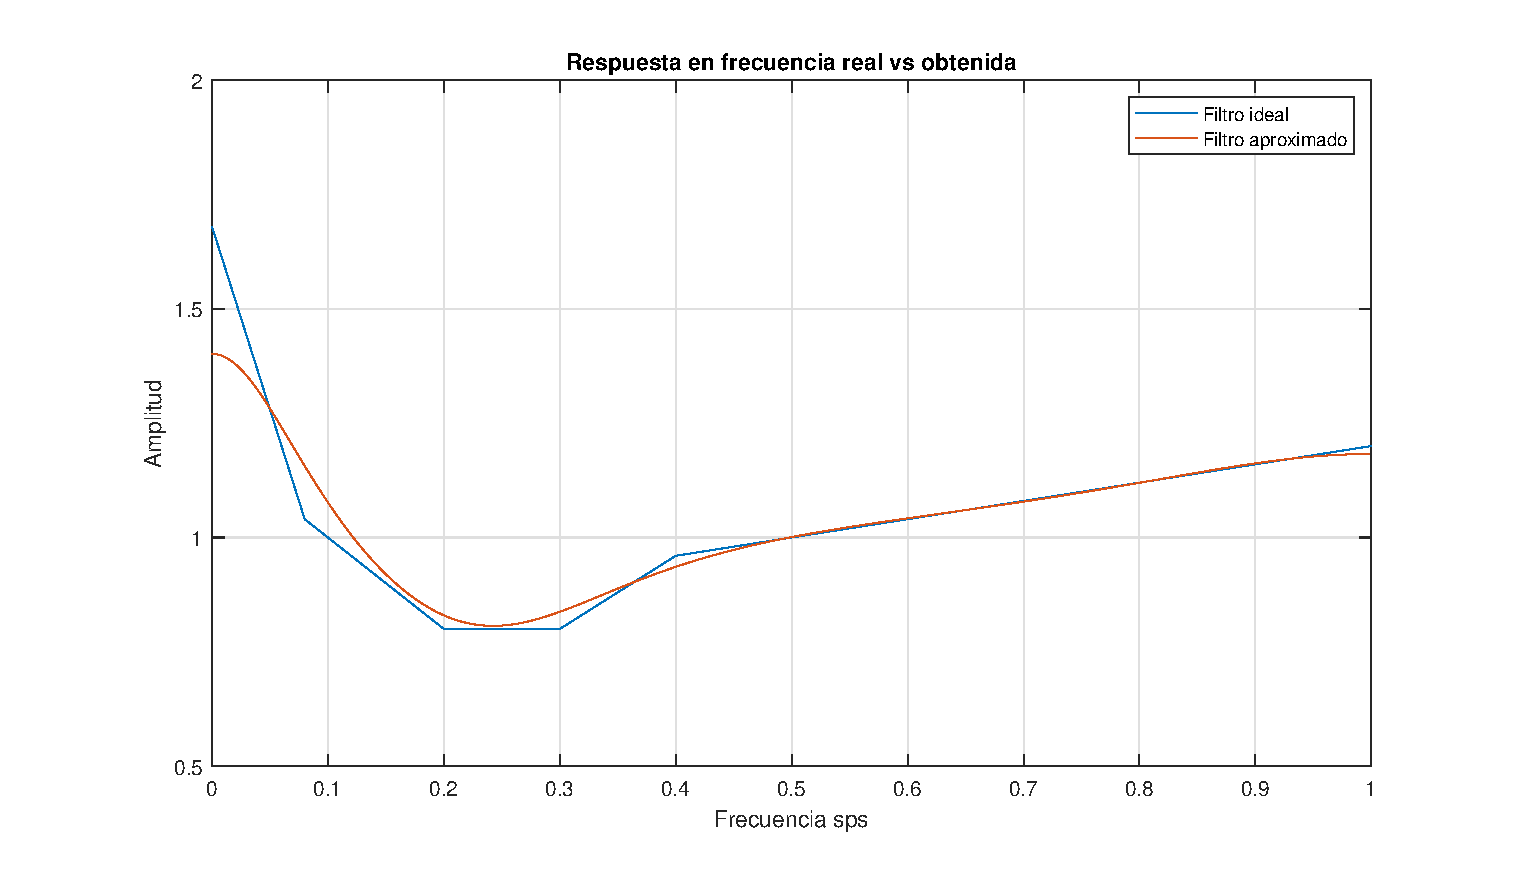
\includegraphics[scale = 0.6]{figures/freqz.eps}
    \caption{Respuestas en frecuencias ideal y obtenida mediante MATLAB}
    \label{freqz}
\end{figure}
    
Los coeficientes para los filtros biquad obtenidos mediante la función \textit{tf2sos} se muestran en la figura \ref{parámetros}

\begin{figure}[H]
    \centering
    \includegraphics[scale = 0.6]{figures/parametros.png}
    \caption{coeficientes obtenidos mediante \textit{tf2sos} para configurar los filtros biquad del \textit{codec} de audio.}
    \label{parámetros}
\end{figure}
    
    
Se debe considerar la discrepancia de signos que se señaló anteriormente para los coeficientes antes de utilizarlos como parámetro en el dispositivo. Además se debe recordar que para poder trabajar dentro del rango adecuado permitido por el dispositivo corrigió la ganancia  del filtro por un factor de 0.8, este efecto se debe corregir y se puede hacer corrigiendo el volumen de salida de audio del dispositivo (tal como se indica en la sección 10.6.1 Output Stage Volume Controls del \textit{datasheet})



\end{enumerate}






\end{document}

